\documentclass[tikz,border=15pt]{standalone}
\usepackage{tikz}
\usepackage{amsmath}
\usepackage{amssymb}
\usetikzlibrary{positioning, arrows.meta, calc, backgrounds, fit, shapes.geometric}

\colorlet{color_shared}{black!70}

\begin{document}

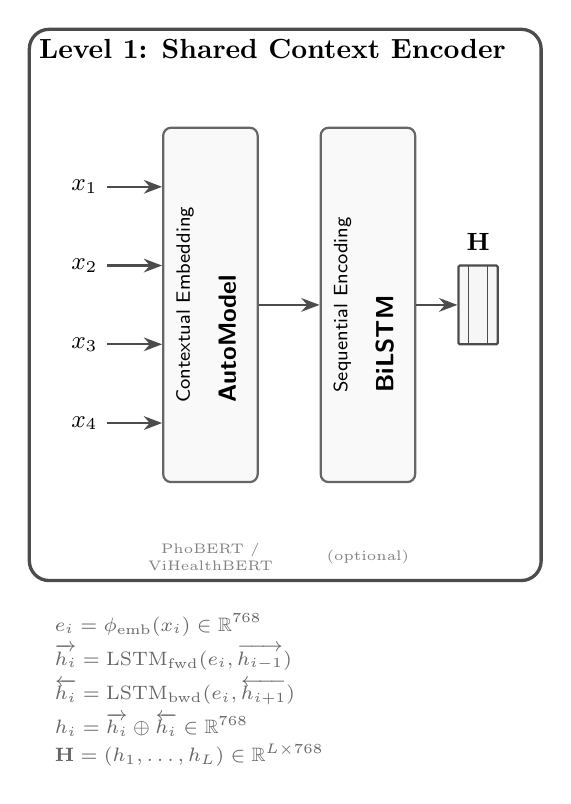
\begin{tikzpicture}[
    >=Stealth, font=\small\sffamily,
    mainbox/.style={draw=black!70, rounded corners=2.5mm, line width=1.2pt},
    block/.style={draw=black!70, fill=white, rounded corners=1mm, thick, align=center},
    shared_block/.style={block, draw=black!60, fill=gray!5},
    arrow/.style={->, thick, draw=black!70},
    matrix_vert/.style={
        draw=#1, thick, fill=#1!5, minimum width=0.5cm, minimum height=1.0cm, rounded corners=0.5pt,
        path picture={
            \draw[#1, thin] (-0.12,-0.5) -- (-0.12,0.5);
            \draw[#1, thin] (0.12,-0.5) -- (0.12,0.5);
        }
    }
]

%% ============================================================
%% TIER 1: SHARED CONTEXT ENCODER
%% ============================================================
\draw[mainbox] (-5.5, 1.5) rectangle (1.0, 8.5);
\node[anchor=north west, font=\bfseries] at (-5.5, 8.5) {Level 1: Shared Context Encoder};

\foreach \i/\y in {1/6.5, 2/5.5, 3/4.5, 4/3.5} {
    \node (x\i) at (-4.8, \y) {$x_{\i}$};
}

\node[shared_block, minimum width=1.2cm, minimum height=4.5cm] (plm) at (-3.2, 5.0) {
    \rotatebox{90}{\scriptsize Contextual Embedding}
    \hspace{0.1cm}
    \rotatebox{90}{\textbf{AutoModel}}
};
\node[font=\tiny, text=black!50, align=center] at (-3.2, 1.8) {PhoBERT /\\ViHealthBERT};
\foreach \i in {1, 2, 3, 4} { \draw[arrow] (x\i) -- (x\i -| plm.west); }

\node[shared_block, minimum width=1.2cm, minimum height=4.5cm] (bilstm) at (-1.2, 5.0) {
    \rotatebox{90}{\scriptsize Sequential Encoding}
    \hspace{0.1cm}
    \rotatebox{90}{\textbf{BiLSTM}}
};
\node[font=\tiny, text=black!50, align=center] at (-1.2, 1.8) {(optional)};
\draw[arrow] (plm.east) -- (bilstm.west);

\node[matrix_vert=color_shared] (H_mat) at (0.2, 5.0) {};
\node[above=0.05cm of H_mat, font=\bfseries\small] {$\mathbf{H}$};
\draw[arrow] (bilstm.east) -- (H_mat.west);

%% --- Equations ---
\node[anchor=north west, font=\scriptsize, text=black!60, align=left] at (-5.3, 1.2) {
    $e_i = \phi_{\text{emb}}(x_i) \in \mathbb{R}^{768}$\\[2pt]
    $\overrightarrow{h_i} = \text{LSTM}_{\text{fwd}}(e_i, \overrightarrow{h_{i-1}})$\\[2pt]
    $\overleftarrow{h_i} = \text{LSTM}_{\text{bwd}}(e_i, \overleftarrow{h_{i+1}})$\\[2pt]
    $h_i = \overrightarrow{h_i} \oplus \overleftarrow{h_i} \in \mathbb{R}^{768}$\\[2pt]
    $\mathbf{H} = (h_1, \dots, h_L) \in \mathbb{R}^{L \times 768}$
};

\end{tikzpicture}

\end{document}
